
% v2-acmsmall-sample.tex, dated March 6 2012
% This is a sample file for ACM small trim journals
%
% Compilation using 'acmsmall.cls' - version 1.3 (March 2012), Aptara Inc.
% (c) 2010 Association for Computing Machinery (ACM)
%
% Questions/Suggestions/Feedback should be addressed to => "acmtexsupport@aptaracorp.com".
% Users can also go through the FAQs available on the journal's submission webpage.
%
% Steps to compile: latex, bibtex, latex latex
%
% For tracking purposes => this is v1.3 - March 2012
\documentclass[prodmode,acmtecs]{acmsmall} % Aptara syntax
\usepackage[spanish,polish]{babel}
\usepackage[T1]{fontenc}
\usepackage{fancyvrb}
\usepackage{graphicx,hyperref}
\newcommand\cutout[1]{}


\usepackage[table]{xcolor}
\usepackage[utf8]{inputenc}
\usepackage[parfill]{parskip}
\usepackage{tabulary}
\PassOptionsToPackage{hyphens}{url}
\usepackage{hyperref}    
\usepackage[capitalize]{cleveref}


% Metadata Information
% !!! TODO: SET THESE VALUES !!!
\acmVolume{0}
\acmNumber{0}
\acmArticle{CFP}
\acmYear{0}
\acmMonth{0}

\newcounter{colstart}
\setcounter{page}{4}

\RecustomVerbatimCommand{\VerbatimInput}{VerbatimInput}%
{
%fontsize=\footnotesize,
fontfamily=\rmdefault
}


\newcommand{\UnderscoreCommands}{%\do\verbatiminput%
\do\citeNP \do\citeA \do\citeANP \do\citeN \do\shortcite%
\do\shortciteNP \do\shortciteA \do\shortciteANP \do\shortciteN%
\do\citeyear \do\citeyearNP%
}

\usepackage[strings]{underscore}



% Document starts
\begin{document}


\setcounter{colstart}{\thepage}

\acmArticle{CFP}
\title{{\huge\sc SIGLOG Monthly 278}

 October 2026}\author{ELLI ANASTASIADI\affil{Aalborg University, SE}\vspace*{-2.6cm}\begin{flushright}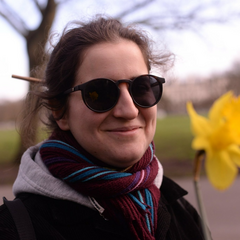
\includegraphics[width=30mm]{elli_anastasiadi.png}\end{flushright}}\begin{abstract}October 2026 edition of SIGLOG Monthly, featuring deadlines, calls and community announcements.
\end{abstract}


\maketitlee

\href{https://lics.siglog.org/newsletters/}{Past Issues}
 - 
\href{https://lics.siglog.org/newsletters/inst.html}{How to submit an announcement}
\section{Table of Contents}\begin{itemize}\item DEADLINES (\cref{deadlines}) 
 
\item CALLS 
 
\begin{itemize}\item AAMAS 2027 (CALL FOR PAPERS) (\cref{AAMAS2027})
\item STACS 2027 (CALL FOR PAPERS ) (\cref{STACS2027})
\item FSEN 2027 (CALL FOR PAPERS ) (\cref{FSEN2027})
\item FSCD and CADE 2027 (CALL FOR WORKSHOPS ) (\cref{FSCDandCADE2027})
\end{itemize} 
\item JOB ANNOUNCEMENTS 
 
\begin{itemize}\item POSTDOC POSITION (\cref{POSTDOCPOSITION})
\end{itemize} 
\end{itemize}\section{Deadlines}\label{deadlines}\rowcolors{1}{white}{gray!25}\begin{tabulary}{\linewidth}{LL}ESSLLI 2027:  & Oct 01, 2026 (Course/workshop titles), Oct 15, 2026 (Course/workshop proposals) \\
AAMAS 2027:  & Oct 01, 2026 (Abstract), Oct 08, 2026 (Paper) \\
STACS 2027:  & Oct 11, 2026 (Submission deadline) \\
FSEN 2027:  & Oct 19, 2026 (Abstract Submission), Oct 28, 2026 (Paper Submission) \\
FSCD and CADE 2027:  & Dec 04, 2026 (Workshop proposal  deadline) \\
DEON 2027:  & Mar 05, 2027 (Abstract), Mar 12, 2027 (Paper) \\
\end{tabulary}
\section{AAMAS 2027: 26th International Conference on Autonomous Agents and Multiagent Systems}\label{AAMAS2027}  3-7 May, Hanoi, Vietnam\\ 
  \href{https://warwick.ac.uk/fac/sci/dcs/aamas2027/}{https://warwick.ac.uk/fac/sci/dcs/aamas2027/}\\ 
CALL FOR PAPERS 

\begin{itemize}\item  We invite submissions to the 26th International Conference on Autonomous Agents and Multiagent Systems (AAMAS 2027), to be held in Hanoi, Vietnam, from 3 to 7 May 2027. Submissions for AAMAS 2027 are on OpenReview: \href{https://openreview.net/group?id=ifaamas.org/AAMAS/2027/Conference}{https://openreview.net/group?id=ifaamas.org/AAMAS/2027/Conference} 
 
\item  IMPORTANT DATES  
 
\rowcolors{1}{white}{gray!25}\begin{tabulary}{\linewidth}{LL}Abstract submission:  & Oct 01, 2026 \\
Paper submission:  & Oct 08, 2026 \\
Rebuttal period:  & Nov, 20-24 2026 \\
Author notification:  & Dec 21, 2026 \\
Camera-ready paper:  & Jan 25, 2027 \\
Conference:  & May, 3-7 2027 \\
\end{tabulary}
 
  All deadlines are at the end of the specified day, Anywhere on Earth (UTC-12).  
 
\item  AAMAS welcomes significant and original research across the full breadth of autonomous agents and multiagent systems, covering established areas as well as emerging topics such as generative and agentic AI. 
 
\item  MORE INFORMATION 
 
\begin{itemize}\item  Conference website: \href{https://warwick.ac.uk/fac/sci/dcs/aamas2027/}{https://warwick.ac.uk/fac/sci/dcs/aamas2027/}
\item  Full Call for Papers: \href{https://warwick.ac.uk/fac/sci/dcs/aamas2027/calls/}{https://warwick.ac.uk/fac/sci/dcs/aamas2027/calls/}
\item  Submission instructions: \href{https://warwick.ac.uk/fac/sci/dcs/aamas2027/calls/instructions/}{https://warwick.ac.uk/fac/sci/dcs/aamas2027/calls/instructions/}
\item  Findings of AAMAS: \href{https://warwick.ac.uk/fac/sci/dcs/aamas2027/calls/findings/}{https://warwick.ac.uk/fac/sci/dcs/aamas2027/calls/findings/}
\end{itemize} 
  Please note that all authors must have an OpenReview account, and abstract registration is required before the full-paper submission deadline. Please refer to the conference website for the complete submission, formatting, reviewing, and publication policies. We look forward to receiving your submissions and to welcoming you to AAMAS 2027 in Hanoi. Please feel free to forward this Call for Papers to colleagues, research groups, and relevant mailing lists. 
 
\item  Call for Reviewer Self-Nominations 
 
  We invite members of the community who are interested in serving as reviewers for AAMAS 2027 to submit a self-nomination through the following form: \href{https://forms.gle/3vd99yvWqNdYqhYR7}{https://forms.gle/3vd99yvWqNdYqhYR7} . We warmly welcome self-nominations across all AAMAS areas. In particular, we would be especially pleased to receive additional nominations in Learning and Adaptation (LEARN), Search, Optimization, Planning, and Scheduling (SOPS), Generative and Agentic AI (GAAI), and Game Theory and Economic Paradigms (GTEP), where strengthening the reviewer pool would be particularly helpful. 
 
  Reviewing is one of the ways in which we collectively sustain the quality of our research community. The broader the participation, the more evenly the workload can be shared, allowing each reviewer to handle a smaller and more manageable set of papers. The form includes the reviewer eligibility requirements and asks for basic OpenReview information and areas of expertise. Candidates who are recruited will subsequently be asked to complete the official Reviewer Registration in OpenReview, which is a separate step in the AAMAS 2027 reviewing workflow. That registration will collect the more detailed expertise information, including area-specific topics, needed for paper matching and assignment. 
 
  Thank you very much for considering contributing to AAMAS 2027. 
 
  Best regards, 
 
  AAMAS 2027 Program Chairs 
 
\item  Reciprocal Reviewer Policy 
 
  Each submission must designate at least one qualified author who agrees to serve as a reviewer for AAMAS. The designated author must meet the qualification criteria defined in the AAMAS Reviewer Guidelines.  
 
\item  Exceptions 
 
\begin{itemize}\item  A submission is exempt from this requirement if:
\item  None of the authors is qualified under the “Reviewer Eligibility section” in the Reviewer Guidelines; or
\item  All qualified authors are serving as Area Chairs (ACs), Senior Program Committee (SPC), or in other official organizing roles for AAMAS 2027.
\item  Read the full policy on the AAMAS website: \href{https://warwick.ac.uk/fac/sci/dcs/aamas2027/calls/reciprocal-reviewer-policy/}{https://warwick.ac.uk/fac/sci/dcs/aamas2027/calls/reciprocal-reviewer-policy/}
\end{itemize} 
\end{itemize}\section{STACS 2027: 44th International Symposium on Theoretical Aspects of Computer Science}\label{STACS2027}  8-12 March, 2027\\ 
  Göttingen, Germany\\ 
  Webpage: \href{https://stacs2027.uni-goettingen.de/}{https://stacs2027.uni-goettingen.de/}\\ 
CALL FOR PAPERS  

  STACS 2027 will consist of two tracks, A and B. Track A (PC chairs: Paweł Gawrychowski, Meirav Zehavi) focuses on algorithms, data structures, and complexity, while track B (PC Chairs: Laurent Bienvenu, Florin Manea) focuses on automata, logic, semantics, and theory of programming. The complete list of the PC can be seen here: \href{https://events.gwdg.de/event/1460/page/472-program-committees}{https://events.gwdg.de/event/1460/page/472-program-committees}\\ 
\begin{itemize}\item  Invited Speakers: 
 
\begin{itemize}\item  Mikołaj Bojańczyk (University of Warsaw)
\item  Jesper Nederlof (Utrecht University)
\end{itemize} 
\item  Tutorial speaker: 
 
\begin{itemize}\item  Inge Li Gørtz (Technical University of Denmark)
\end{itemize} 
\item  Submissions: 
 
  For all details (including instructions regarding AI usage), see the webpage \href{https://events.gwdg.de/event/1460/page/476-submissions}{https://events.gwdg.de/event/1460/page/476-submissions}. Quick overview: 
 
  Authors are invited to submit papers presenting original and unpublished research on theoretical aspects of computer science. Topics covered by the tracks include, but are not limited to, the following:                    
 
\begin{itemize}\item  Track A. Algorithms, Data Structures, and Complexity                         
\item  Track B. Automata, Logic, Semantics and Theory of Programming
\end{itemize} 
\item  IMPORTANT DATES 
 
\rowcolors{1}{white}{gray!25}\begin{tabulary}{\linewidth}{LL}Submission deadline:  & Oct 11, 2026 \\
Rebuttal:  & Nov 30 -Dec 2, 2026 \\
Notification:  & Dec 22, 2026 \\
Conference:  & Mar, 8-12 2027 \\
\end{tabulary}
 
\item  Format of submissions: 
 
  Submissions should be made through EasyChair at \href{https://easychair.org/conferences/?conf=stacs2027}{https://easychair.org/conferences/?conf=stacs2027} Authors are invited to submit an extended abstract or a full paper with at most 15 pages; this page limit excludes the title page, the references section, and a possible appendix. In preparing submissions, the usage of the LIPIcs style file is mandatory; no changes to font size, page geometry, etc. are permitted. Please refer to LIPIcs author instructions. Submissions submitted after the deadline will not be considered, and submissions not adhering to the expected format risk rejection without consideration of the content. Submissions should be made to appropriate tracks. The PCs reserve the right to reassign a paper to a different track, if deemed necessary. 
 
  The extended abstract should contain a succinct statement of the considered issues and of their motivation, a summary of the main results, and a brief explanation of their significance, accessible to non-specialist readers. This should be followed by a rigorous derivation of the claimed results. Proofs omitted due to space constraints should be put into an appendix. It is allowed and encouraged to provide the anonymized full version of the paper as the appendix. Simultaneous submission to other conferences with published proceedings or to journals is not allowed. PC members are allowed to submit their works as well, except for PC chairs.                                                            
 
\item  Double-blind reviewing: 
 
  As in the previous years, STACS 2027 will employ a lightweight double-blind reviewing process: submissions should not reveal the identity of the authors in any way. Nothing should be done in the name of anonymity that weakens the submission or makes the job of reviewing the paper more difficult. In particular, important references should not be omitted or anonymized. In addition, authors should feel free to disseminate their ideas or draft versions of their paper as they normally would. For example, authors may post drafts of their papers on the web, submit them to arXiv, and give talks on their research ideas. 
 
\item  Rebuttal:                                              
 
  There will be a rebuttal period for authors. Authors will receive the reviews of their submissions and have a few days to prepare and submit rebuttals. These rebuttals become part of the PC discussions, but entail no specific responses. Rebuttals will be handled through EasyChair.                                                      
 
\item  At least one author of each accepted paper is expected to register at the conference. For authors who cannot present their paper in person, a possibility for remote presentation will be offered.    
 
\end{itemize}\section{FSEN 2027: Twelfth International Conference on Fundamentals of Software Engineering 2027 - Theory and Practice}\label{FSEN2027}  \href{https://conf.researchr.org/home/fsen-2027}{https://conf.researchr.org/home/fsen-2027}\\ 
  University of Twente, Enschede, the Netherlands\\ 
  May 24-25, 2027\\ 
CALL FOR PAPERS  

\begin{itemize}\item  ABOUT FSEN 
 
  Fundamentals of Software Engineering (FSEN) is an international conference that aims to bring together researchers, engineers, developers, and practitioners from academia and industry to present and discuss their research work in the area of formal methods for software engineering. Additionally, this conference seeks to facilitate the transfer of experience, adaptation of methods, and where possible, foster collaboration among different groups. The topics of interest cover all aspects of formal methods, especially those related to advancing the application of formal methods in the software industry and promoting their integration with practical engineering techniques. Following the success of the previous FSEN editions, the next edition of the FSEN conference will take place at the University of Twente, in Enschede, the Netherlands, May 24-25, 2027. 
 
\item  IMPORTANT DATES 
 
\rowcolors{1}{white}{gray!25}\begin{tabulary}{\linewidth}{LL}Abstract Submission:  & Oct 19, 2026 \\
Paper Submission:  & Oct 28, 2026 \\
Notification:  & Dec 18, 2026 \\
Pre-conference Camera-ready Submission:  & Feb 22, 2027 \\
Poster Submission:  & Feb 24, 2027 \\
Conference:  & May 24-25, 2027 \\
\end{tabulary}
 
\item  KEYNOTE SPEAKERS 
 
\begin{itemize}\item  Jan Friso Groote, Eindhoven University of Technology, Netherlands
\item  Paula Herber, University of Munster, Germany
\item  Laura Kovács, Vienna University of Technology, Austria
\item  Ivo ter Horst, ASML, Netherlands
\end{itemize} 
\item  For a full list of topics of interest please visit the online call for papers 
 
\item  PAPER SUBMISSION  
 
  Authors are invited to submit: 
 
\begin{itemize}\item  Full papers (up to 16 pages excluding references) describing original research, applications and tools;
\item  Short papers (up to 6 pages excluding references) describing ongoing research or new ideas that have not yet been fully validated;
\item  Posters (up to 4 pages excluding references) describing ongoing work.
\end{itemize} 
  At least one of the authors should register and present the paper at the conference. Upon request, up to five papers can be accepted by the PC for which no presence on site is required. 
 
\item  FSEN'27 will follow a single-blind reviewing process. Appendices are optional and will not be included in the proceedings. All categories of papers must be submitted electronically in PDF using the online submission process via the EasyChair conference system at the following link: \href{https://www.easychair.org/conferences/?conf=fsen2027}{https://www.easychair.org/conferences/?conf=fsen2027}. 
 
  Contributions must be written in English, should be formatted according to the Springer LNCS style (LaTeX2e Proceedings Templates) that can be found at the following link (\href{http://www.springer.com/gp/computer-science/lncs/conference-proceedings-guidelines}{http://www.springer.com/gp/computer-science/lncs/conference-proceedings-guidelines}) and not exceed the page limit for the category (including figures and references). Submissions should use default font sizes and margins, and be in A4 paper size. 
 
  Each submission will be thoroughly reviewed by at least three reviewers considering scientific originality, significance, relevance to the FSEN conference, technical soundness, clarity, self-containedness and discussion of appropriate related work. 
 
  The reviewers will be asked to rate the submissions and evaluate whether they can be accepted as: 
 
\begin{itemize}\item  Full paper for the LNCS proceedings
\item  Short paper for the LNCS proceedings
\item  Poster (not included in the proceedings)
\end{itemize} 
  Papers accepted in the first two categories will be invited for presentation at the conference. Posters will be illustrated by the authors in separate poster sessions. 
 
\item  Responsible use of generative AI 
 
  Following the tradition of previous editions of FSEN, the proceedings will published in the LNCS series of Springer. We therefore recommend to carefully check the Springer policy regarding the use of generative AI. In brief this policy does allow for the use of AI tools to support the preparation of the manuscript, but authors must ensure that human expertise is involved in the editing and fact-checking of AI-generated content. Authors must transparently declare any use of AI tools in their manuscripts and are fully responsible for the content and integrity of their work, provided that the intellectual contributions—such as ideas, analysis, and conclusions—are original and human-generated; AI cannot be listed as an author or co-author. We further expect responsible use of AI and that authors commit themselves to maintain the integrity of scholarly communication. We also require reviewers to adhere to the non-disclosure of submitted manuscripts. This includes the requirement that reviews are being performed by the reviewers themselves and that submitted manuscripts are not being uploaded to AI tools. The use of tools for correcting spelling and grammar of the review reports themselves is permitted. 
 
  For further details or specific issues regarding the AI policies of associations supporting FSEN and Springer, please consult: 
 
\begin{itemize}\item  Springer’s policies and guidances for AI (\href{https://group.springernature.com/gp/group/ai/ai-guidance-for-our-researchers-and-communities}{https://group.springernature.com/gp/group/ai/ai-guidance-for-our-researchers-and-communities})
\item  Springer’s Code of Conduct (\href{https://www.springernature.com/gp/authors/book-authors-code-of-conduct}{https://www.springernature.com/gp/authors/book-authors-code-of-conduct})
\item  IFIP's Code of Ethics/Conduct (\href{https://www.ifip.org/ifip-code-of-ethics/}{https://www.ifip.org/ifip-code-of-ethics/})
\item  ACM's Policy on Authorship (\href{https://www.acm.org/publications/policies/new-acm-policy-on-authorship}{https://www.acm.org/publications/policies/new-acm-policy-on-authorship})
\end{itemize} 
\item  Proceedings and Special Issue 
 
  The proceedings of FSEN'27 will be published by Springer in the LNCS series. Following the tradition of FSEN, we plan to have a special issue of the Science of Computer Programming journal devoted to FSEN'27. After the conference a selection of papers will be invited for this special issue. The invited papers should be revised and extended and will undergo a new round of review by an international program committee. Please see the websites of previous editions of FSEN for more information on proceedings and special issues related to those editions. 
 
\item  GENERAL CHAIRS  
 
\begin{itemize}\item  Mieke Massink, CNR-ISTI, Pisa, Italy
\item  Mariëlle Stoelinga, University of Twente, Enschede, and Radboud University, Nijmegen, the Netherlands
\end{itemize} 
\end{itemize}\section{FSCD and CADE 2027: }\label{FSCDandCADE2027}  21-27 August, 2027\\ 
  Nijmegen, the Netherlands\\ 
  \href{https://fscd-cade.science.ru.nl/}{https://fscd-cade.science.ru.nl/}\\ 
CALL FOR WORKSHOPS  

\begin{itemize}\item  CADE and FSCD 2027 will take place in Nijmegen from 22nd to 26th August 2027. We invite proposals of interest to either community.  Proposals must be limited to three pages, and should be submitted to Cynthia Kop <C.Kop@cs.ru.nl>. 
 
\item  Proposals should include: 
 
\begin{itemize}\item  the workshop's name and URL if already available (or from previous years)
\item  which conference you mean to affiliate with (CADE, FSCD or both)
\item  a short scientific summary of the workshop's topic
\item  a list of workshop organisers with contact information
\item  procedure for selecting presentations (e.g., contributing talks, speaker invitations)
\item  proposed duration (e.g., 1/2, 1, 1.5 or 2 days)
\item  expected number of in-person participants, providing some data on previous years if the workshop has already been organised in the past
\item  special resources that may be required (e.g., a room for posters)
\item  preferred dates (see below)
\item  any other relevant information and special wishes about the schedule (e.g., avoiding overlap with certain other workshops or business meetings)
\end{itemize} 
  Proposals for other colocated events, such as poster sessions or competitions, should be submitted in the same way. 
 
  The available dates are in principle: 
 
\begin{itemize}\item  Saturday 21 and Sunday 22 August for FSCD workshops, with an option for 27 August in case there are many workshops.
\item   Saturday 21 and Thursday 26 August for CADE workshops, with an option for 27 August in case there are many workshops, or two-day workshops.
\end{itemize} 
  However, on request, we may also schedule workshops / poster sessions / competitions /during/ their affiliated conference (22-25 August for CADE and 23-26 August for FSCD) instead of before/after. 
 
\item  IMPORTANT DATES 
 
\rowcolors{1}{white}{gray!25}\begin{tabulary}{\linewidth}{LL}Workshop proposal submission deadline:  & Dec 04, 2026 \\
Notification:  & Jan 01, 2027 \\
\end{tabulary}
 
\end{itemize}\section{POSTDOC POSITION: School of Computer Science, University of Sydney, Australia}\label{POSTDOCPOSITION}JOB ANNOUNCEMENT 

  A postdoctoral position in theoretical computer science is available with Sasha Rubin at the University of Sydney on topics related to reactive synthesis and nondeterministic planning. The appointment is funded by the ARC project “Logic-based planning under ignorance”. The appointment is expected to start in 2027, initially for two years with the possibility of extension. The successful candidate will join the Sydney Algorithms and Computing Theory group working in foundational aspects of computer science (usyd-sact.github.io/). Application link: tinyurl.com/cmfe4s58 For informal inquiries, feel free to contact me at sasha.rubin@sydney.edu.au\\ 



\bigskip Links: \href{http://siglog.org/}{SIGLOG website}, \href{https://lics.siglog.org}{LICS website}, \href{https://lics.siglog.org/newsletters/}{SIGLOG Monthly}\end{document}